%%%% Paramétrage du TD %%%%
\def\xxactivite{\ifcolle Colle \else TD 1 \fi  \ifprof -- Corrigé \else \fi} % \normalsize \vspace{-.4cm}
\def\xxauteur{\textsl{Xavier Pessoles}}

\def\xxnumchapitre{Chapitre 3 \vspace{.2cm}}
\def\xxchapitre{\hspace{.12cm} Méthodologie : détermination des équations de mouvement}
\def\xxpartie{Modéliser le comportement des systèmes mécaniques dans le but d'établir une loi de comportement ou de déterminer des actions mécaniques en utilisant le PFD}



\def\xxtitreexo{Dynamique du véhicule -- Chariot élévateur à bateaux\ifnormal $\star$ \else \fi \ifdifficile $\star\star$ \else \fi \iftdifficile $\star\star\star$ \else \fi }

\def\xxsourceexo{\hspace{.2cm} \footnotesize{X -- ENS -- PSI -- 2012}}


\def\xxcompetences{%
\vspace{-.5cm}
\textsl{%
\textbf{Savoirs et compétences :}
\begin{itemize}[label=\ding{112},font=\color{ocre}] 
%\item \textit{Mod2.C16} : torseur cinétique
%\item \textit{Mod2.C17} : torseur dynamique
%\item \textit{Mod2.C17.SF1} : déterminer le torseur dynamique d’un solide, ou d’un ensemble de solides, par rapport à un autre solide
%\item \textit{Mod2.C15} : matrice d'inertie
\item \textit{Res1.C2} : principe fondamental de la dynamique
\item \textit{Res1.C1.SF1} : proposer une démarche permettant la détermination de la loi de mouvement
%\item \textit{Res1.C2.SF1} : proposer une méthode permettant la détermination d’une inconnue de liaison
\end{itemize}
}}
\def\xxfigures{
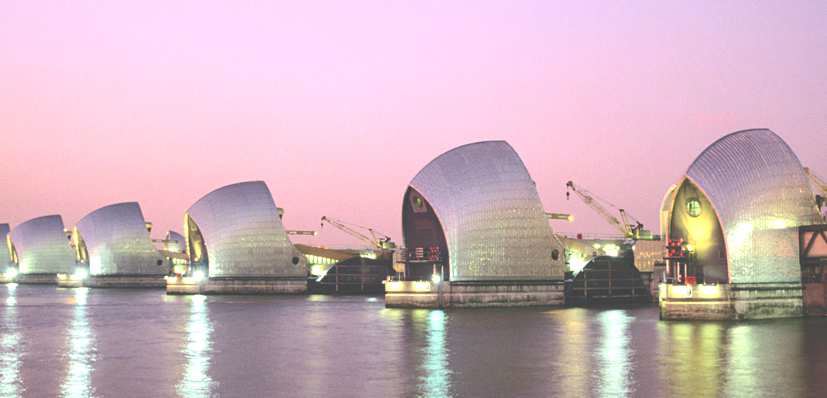
\includegraphics[width=.55\linewidth]{fig_00}
}%figues de la page de garde


\input{\repRel/Style/pagegarde_TD}
\setcounter{numques}{0}

\setlength{\columnseprule}{.1pt}

\pagestyle{fancy}
\thispagestyle{plain}

\ifprof
\vspace{4.8cm}
\else
\vspace{4.8cm}
\fi

\def\columnseprulecolor{\color{ocre}}
\setlength{\columnseprule}{0.4pt} 

%%%%%%%%%%%%%%%%%%%%%%%

\setcounter{exo}{0}

\ifprof
%\begin{multicols}{2}
\else
\begin{multicols}{2}
\fi

\subsection*{Présentation}

\ifprof
\else
Le chariot élévateur , objet de cette étude,  permet la manutention de bateaux de \SI{3000}{kg}
à une hauteur de \SI{8}{m}. Il est principalement constitué :
\begin{itemize}
\item du chariot qui assure le déplacement de l’ensemble et apporte la puissance pour la préhension
et le levage ;
\item du tablier, constitué du mât et des fourches, qui permet la préhension et la dépose du bateau.
\end{itemize}

\begin{center}
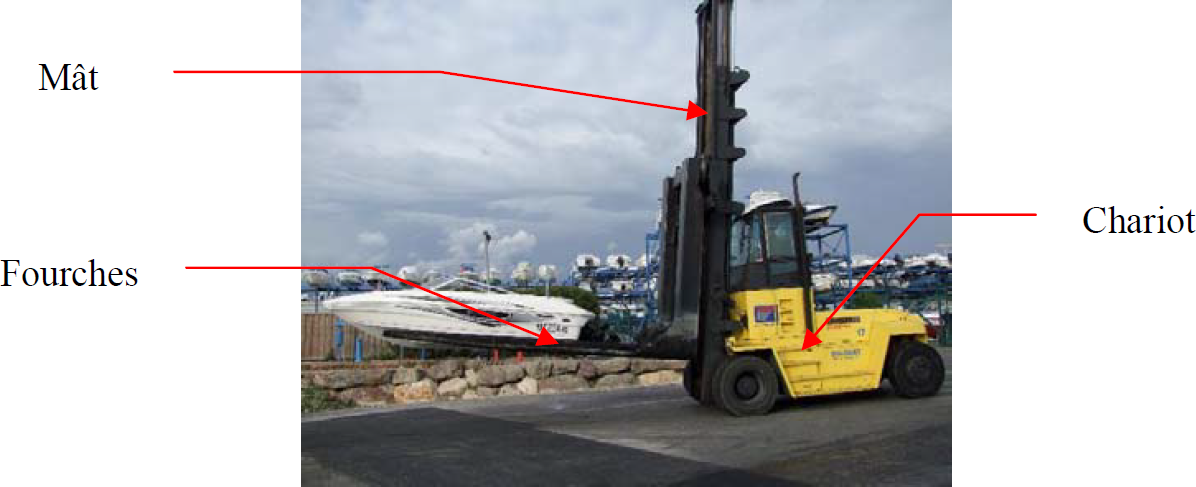
\includegraphics[width=\linewidth]{fig_01a}
\end{center} 
On considère que le chariot élévateur se déplace sur le trajet de référence de la Figure 1. Les basculements frontal et latéral des chariots élévateurs représentent le principal risque auquel est confronté le conducteur. L’objectif de cette partie est de définir les conditions de stabilité du chariot élévateur dans les phases de freinage et lors des virages afin de définir les conditions optimales de déplacement du chariot dans chacune des phases.
La caractérisation partielle de l'exigence 2 est donnée sur la Figure 2.



\begin{center}
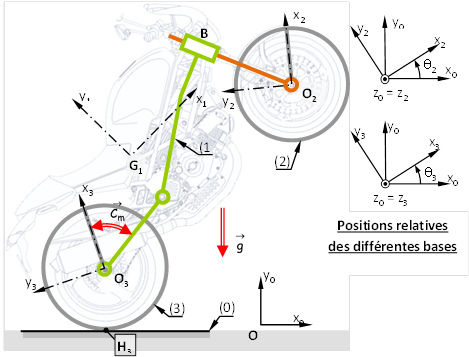
\includegraphics[width=.8\linewidth]{fig_01}
\end{center}

\begin{center}
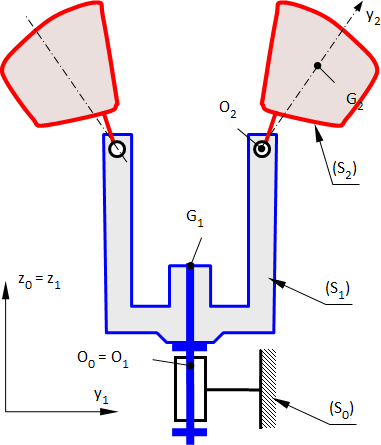
\includegraphics[width=\linewidth]{fig_02}
\end{center}

\begin{obj}
L'objectif est de valider l'exigence suivante : << req 2 : le conducteur peut déplacer le bateau en toute sécurité >>. 
\end{obj}
\fi

\subsection*{Étude de la position du centre de gravité}
\ifprof
\else
La position du centre de gravité de l’ensemble « chariot+tablier » influence directement la stabilité lors des déplacements. Il est impératif de connaître avec précision sa position.
Étant donné qu’il est possible de monter, sur le même chariot, différents types de tabliers en fonction de l’utilisation souhaitée, le chariot est équipé d’un contrepoids qui permet de régler la position du centre de gravité de l’ensemble. Ce réglage est effectué en usine et dépend du contexte d’utilisation du chariot élévateur.
\fi

\begin{obj}
L'objectif est de valider l'exigence suivante : << req C206 : la position du centre de gravité de l'ensemble $\Sigma$=\{chariot, tablier, contrepoids\} doit être situé à un tiers de l'empattement par rapport à l'axe des roues arrières>>. 
\end{obj}

\ifprof
\else
La Figure suivante donne le paramétrage retenu pour l’étude. On note $\rep{1}=\repere{O}{x_1}{y_1}{z_1}$ le repère lié au chariot. Le plan $\left(O,\vect{x_1},\vect{z_1} \right)$ est un plan de symétrie matériel pour le chariot.

\begin{center}
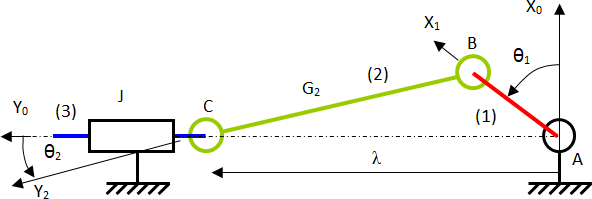
\includegraphics[width=\linewidth]{fig_03}
\end{center}

Le repère  $\rep{0}=\repere{O_0}{x_0}{y_0}{z_0}$ est un repère lié à la route, supposé galiléen pour les conditions de l’étude.

On note : 
\begin{itemize}
\item $G_B$ : centre de gravité du bateau de masse $m_B$;
\item $G_T$ : centre de gravité du tablier de masse $m_T$;
\item $G_1$ : centre de gravité du chariot seul de masse $m_1$;
\item $G_C$ : centre de gravité du contrepoids de masse $m_C$;
\item $G$ : centre de gravité de l'ensemble $\Sigma =  \{\text{chariot, tablier, contrepoids}\}$.
\end{itemize}

On donne : 
$\vect{OG_B}=\begin{pmatrix}x_{G_B} \\ 0 \\ z_{G_B}\end{pmatrix}_{\rep{1}}$,
$\vect{OG_T}=\begin{pmatrix}x_{G_T} \\ 0 \\ z_{G_T}\end{pmatrix}_{\rep{1}}$,
$\vect{OG_1}=\begin{pmatrix}x_{G_1} \\ 0 \\ z_{G_1}\end{pmatrix}_{\rep{1}}$,
$\vect{OG_C}=\begin{pmatrix}x_{G_C} \\ 0 \\ z_{G_C}\end{pmatrix}_{\rep{1}}$.

Afin de minimiser les risques de basculement du chariot élévateur, on souhaite que le point $G$ soit
confondu avec le point $O$ (exigence req C206).
\fi


\question{Déterminer l’expression de $x_{G_C}$ afin de valider l'exigence req C206.}
\ifprof
\begin{corrige}
On a $\vect{OG}=\dfrac{m_T}{m_T+m_1+m_C}\vect{OG_T}+\dfrac{m_1}{m_T+m_1+m_C}\vect{OG_1}+\dfrac{m_C}{m_T+m_1+m_C}\vect{OG_C}$. On souhaite que $\vect{OG}=\vect{0}$. 
On a donc $0=\dfrac{m_T}{m_T+m_1+m_C}x_{G_T}+\dfrac{m_1}{m_T+m_1+m_C}x_{G_1}+\dfrac{m_C}{m_T+m_1+m_C}x_{G_C}$ et donc : $x_{G_C}=-\dfrac{m_T}{m_C}x_{G_T}-\dfrac{m_1}{m_C}x_{G_1}$.
\end{corrige}
\else
\fi


Pour toute la suite de l’étude, les points $G$ et $O$ sont supposés confondus et la masse totale de
l’ensemble $\Sigma =  \{\text{chariot, tablier, contrepoids}\}$ est notée $M$.

\subsection*{Étude du basculement frontal}
\ifprof
\else
Afin d’éviter les risques de basculement frontal du chariot lors des phases de freinage, le dispositif de
sécurité ADS permet au conducteur de choisir, à partir des commandes disponibles sur son tableau de
bord, la valeur de la décélération à imposer au chariot avant l’arrêt total. Ainsi, lorsque le conducteur
relâche complètement la pédale de l’accélérateur, le dispositif ADS entre en action et le chariot est
alors animé d’un mouvement uniformément décéléré. Le choix de la valeur de la décélération est fait
en fonction des conditions de chargement du chariot. Ce dispositif permet au conducteur de maîtriser
parfaitement les distances d’arrêt tout en évitant le basculement frontal.

L’objectif de cette partie est de mettre en évidence l’intérêt d’un tel dispositif.

Le chariot est en phase de freinage sur une route horizontale, il transporte un bateau (B) de masse $m_B$
et de centre de gravité $G_B$. La vitesse du centre de gravité de l’ensemble $\Sigma$ est donnée par
$\vectv{G}{\Sigma}{\rep{0}}=V(t)\vect{x_1}$. Tous les mouvements du tablier sont inactifs durant le déplacement. Il n’y a pas de mouvement relatif entre le bateau et l’ensemble $\Sigma$ au cours de cette phase.
L’objet est de déterminer la valeur de la décélération qui provoque le basculement frontal de
l’ensemble $\{\Sigma , B\}$.
Le problème est traité en trois dimensions.

L'action mécanique exercée par le sol sur le pneu $P_i$ est modélisée par le torseur $\torseurstat{T}{\text{sol}}{P_i}=\torseurl{\vectf{\text{sol}}{P_i}=-T_i\vect{x_1}+N_i\vect{z_1}}{\vectm{I_i}{\text{sol}}{P_i}=\vect{0}}{I_1}=\torseurcol{-T_i}{0}{N_i}{0}{0}{0}{I_i,\rep{1}}$.

La masse et l’inertie des roues sont négligées. La décélération qui provoque le basculement de l’ensemble $\{\Sigma, B\}$ est notée $\vect{\Gamma_{\text{dec}}}\left( \{ \Sigma,B\}/\rep{0}\right)=-\text{dec}_x\vect{x_1}$

On admet, dans un premier temps, que le basculement a lieu avant le glissement. Cette hypothèse sera
vérifiée par la suite.

\fi

\question{Écrire les équations issues de l’application du principe fondamental de la dynamique à
l’ensemble $\{\Sigma , B\}$ . Le théorème du moment dynamique sera appliqué au point $I_4$.}
\ifprof
\begin{corrige}
\textbf{On  isole $\{\Sigma , B\}$.}

\textbf{On fait le BAME.}

\begin{itemize}
\item Poids du bateau : $\torseurstat{T}{\text{pes}}{B}=\torseurl{-m_Bg\vect{z}}{\vect{0}}{O}=\torseurl{-m_Bg\vect{z}}{m_Bg\vect{y}\left(x_{G_B}-\dfrac{2L}{3} \right)+Em_Bg\vect{x}}{I_4}$. 
\item Poids de $\Sigma$ : $\torseurstat{T}{\text{pes}}{\Sigma}=\torseurl{-Mg\vect{z}}{\vect{0}}{O}=\torseurl{-Mg\vect{z}}{-\dfrac{2MgL}{3}\vect{y}+EMg\vect{x}}{I_4}$. 
\item Action du sol sur chaque roue : 
\begin{itemize}
\item  $\torseurstat{T}{\text{sol}}{P_1}$ $=\torseurl{-T_1\vect{x}+N_1\vect{z}}{LN_1\vect{y}}{I_4}$;
\item  $\torseurstat{T}{\text{sol}}{P_2}$ $=\torseurl{-T_1\vect{x}+N_1\vect{z}}{-2EN_2\vect{x}+LN_2\vect{y}-2ET_2\vect{z}}{I_4}$;
\item  $\torseurstat{T}{\text{sol}}{P_3}$ $=\torseurl{-T_3\vect{x}+N_3\vect{z}}{-2EN_3\vect{x}-2ET_3\vect{z}}{I_4}$;
\item  $\torseurstat{T}{\text{sol}}{P_4}$ $=\torseurl{-T_4\vect{x}+N_4\vect{z}}{\vect{0}}{I_4}$.
\end{itemize}
\end{itemize}

\textbf{Calcul du $\torseurdyn{\{\Sigma , B\}}{0}$.}

$\torseurdyn{\{\Sigma , B\}}{0} = \torseurl{\vectrd{\{\Sigma , B\}}{0}}{\vectmd{I_4}{\{\Sigma , B\}}{0}}{I_4}$. 

On a $\vectrd{\{\Sigma , B\}}{0}=-\left(M+m_B\right) \text{dec}_x\vect{x_1}$.

Par ailleurs, on a $\vectmd{G}{\{\Sigma , B\}}{0}= \vectmd{G}{\Sigma }{0}+\vectmd{G}{ B}{0}$.
Le bateau étant en translation par rapport au bâti, on a donc :

\begin{itemize}
\item  $\vectmd{G}{\{\Sigma \}}{0}=\vect{0}$ et 
$\vectmd{I_4}{\{\Sigma \}}{0}=\vectmd{G}{\{\Sigma ,\}}{0}+\vect{I_4 G} \wedge \vectrd{\{\Sigma \}}{0} $ $ =\left(-2\dfrac{L}{3} \vect{x_1}-E\vect{y_1}+h\vect{z_1} \right)\wedge -M\text{dec}_x \vect{x_1}=-M\text{dec}_x \left(E\vect{z_1}+h\vect{y_1}\right)$;
\item  $\vectmd{G_B}{\{ B\}}{0}=\vect{0}$ et 
$\vectmd{I_4}{\{ B\}}{0}=\vectmd{G_B}{\{ B\}}{0}+\vect{I_4 G_B} \wedge \vectrd{\{ B\}}{0} $ $=\left(\left(-x_{G_B}+2\dfrac{L}{3}\right) \vect{x_1}+E\vect{y_1}+\left(z_{G_B}+h\right) \vect{z_1} \right)\wedge -m_B \text{dec}_x \vect{x_1}=m_B \text{dec}_x \left(E\vect{z_1}-\left(z_{G_B}+h\right) \vect{y_1}\right)$; 
\item au final, $\vectmd{I_4}{\{\Sigma , B\}}{0}=m_B \text{dec}_x \left(E\vect{z_1}-\left(z_{G_B}+h\right) \vect{y_1}\right)-M\text{dec}_x \left(E\vect{z_1}+h\vect{y_1}\right)$.
\end{itemize}

\textbf{On applique le PFD.}
\begin{itemize}
\item Théorème de la résultante dynamique :
\begin{itemize}
\item suivant $\vect{x_1}$ :$-\left(M+m_B\right) \text{dec}_x=-\sum\limits_{i=1}^{4} T_i$;
\item suivant $\vect{y_1}$ :$0=0$;
\item suivant $\vect{z_1}$ :$0=\sum\limits_{i=1}^{4} N_i-\left(M+m_B\right)g$.
\end{itemize}
\item Théorème du moment dynamique:
\begin{itemize}
\item suivant $\vect{x_1}$ :$0=Em_B g+EM g-2EN_2-2EN_3 $;
\item suivant $\vect{y_1}$ :$-m_B \text{dec}_x \left(z_{G_B}+h\right)-M\text{dec}_x h=L\left(N_1+N_2 \right)+m_B g\left(x_{G_B}-2\dfrac{L}{3}\right)-\dfrac{M g2L}{3} $;
\item suivant $\vect{z_1}$ :$ m_B \text{dec}_x E-M\text{dec}_x E=-2ET_2-2ET_3$.
\end{itemize}
\end{itemize}


\end{corrige}
\else
\fi

\question{Donner les hypothèses qui peuvent être faites afin de réduire le nombre d’inconnues du
problème.}
\ifprof
\begin{corrige}
La mise en équation précédente permet d'exprimer 8 inconnues ($N_i$ et $T_i$ pour $i$ allant de 1 à 4).

En faisant l'hypothèse que le plan $\left(G_1,\vect{z_1},\vect{x_1}\right)$ est plan de symétrie, on peut considérer que $N_4=N_3$, $T_4=T_3$, $N_1=N_2$, $T_1=T_2$. Il reste donc 4 inconnues. 

De plus, à la limite du basculement frontal, les roues arrières se décolleraient. Il resterait donc les inconnues $N_3$ et $T_3$. 
\end{corrige}
\else
\fi

On considère que le basculement a lieu lorsque les roues arrière perdent le contact avec le sol.

\question{Déterminer alors l’expression de $\text{dec}_x$.}
\ifprof
\begin{corrige}
Le basculement frontal du véhicule peut se traduire par un théorème du moment dynamique appliqué en $I_4$ en projection sur $\vect{y_1}$. On utilise les conditions précédentes. On a donc : 
 
 $-m_B \text{dec}_x \left(z_{G_B}+h\right)-M\text{dec}_x h=m_B g\left(x_{G_B}-2\dfrac{L}{3}\right)-\dfrac{M g2L}{3}$ soit 
 $\text{dec}_x  = \dfrac{m_B g\left(x_{G_B}-2\dfrac{L}{3}\right)-\dfrac{M g2L}{3}}{-m_B  \left(z_{G_B}+h\right)-M h}$
 
 $ \Leftrightarrow \text{dec}_x  = -g\dfrac{m_B \left(3x_{G_B}-2L\right)-M 2L}{3m_B  \left(z_{G_B}+h\right)+3M h}$
\end{corrige}
\else
\fi

Le facteur d’adhérence entre le pneu et la route est noté $f$ .

\question{Donner les expressions de $N_4$ et $T_4$ et expliquer qualitativement comment vérifier que le
basculement a lieu avant le glissement afin de justifier l’hypothèse faite en début d’étude.}
\ifprof
\begin{corrige}
\end{corrige}
\else
\fi


\subsection*{Étude du basculement latéral}

\ifprof
\else

Le centre de gravité de l’ensemble $\{\Sigma , B\}$ est noté $G_{\Sigma B}$ $\vect{OG_{\Sigma B}}\begin{pmatrix}x_{G_{\Sigma B}}\\y_{G_{\Sigma B}}\\z_{G_{\Sigma B}} \end{pmatrix}_{\rep{1}}$.


L’objet est de déterminer la vitesse maximale avec laquelle le chariot peut aborder le virage sans
risque de basculement latéral.
Le schéma retenu pour l’étude est présenté sur la Figure 24.
Le chariot aborde un virage de rayon de courbure $\rho$ avec $\vect{O_0G_{\Sigma B}}=-\rho \vect{y_1}$.Tous les mouvements du
tablier sont inactifs durant le déplacement. Il n’y a pas de mouvement relatif entre le bateau B et
l’ensemble $\Sigma$ au cours du mouvement.
La vitesse du chariot est constante pendant toute la phase de virage et est notée $\vectv{G}{\Sigma}{\rep{0}}=V\vect{x_1}$.
La masse et l’inertie des roues sont négligées.
On admet que le basculement latéral a lieu avant le glissement, cette hypothèse pourra être vérifiée par
la suite.

\begin{center}
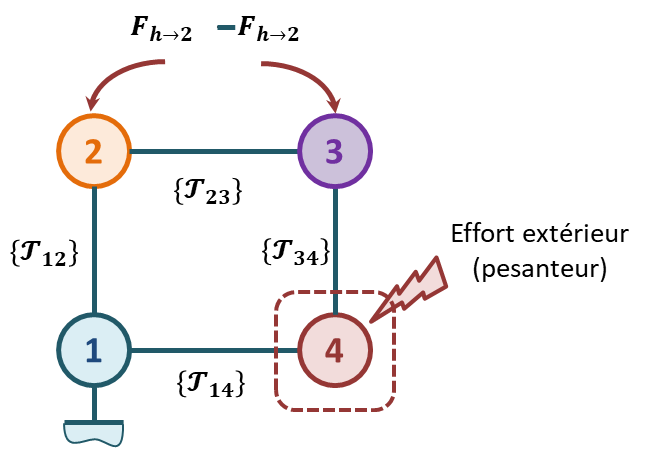
\includegraphics[width=\linewidth]{fig_04}
\end{center}


Le rayon de courbure du virage $\rho$ est suffisamment grand devant l’empattement $E$ du chariot pour
pouvoir négliger l’influence du braquage des roues dans le modèle proposé. L’action mécanique
exercée par le sol sur le pneu $i$ est modélisée par le torseur :
$\torseurstat{T}{\text{sol}}{P_i}=\torseurl{\vectf{\text{sol}}{P_i}=-T_i\vect{x_1}+N_i\vect{z_1}}{\vectm{I_i}{\text{sol}}{P_i}=\vect{0}}{I_1}=\torseurcol{-T_i}{0}{N_i}{0}{0}{0}{I_i,\rep{1}}$.


La matrice d'inertie de l'ensemble $\{\Sigma, B\}$ est de la forme $\inertie{G_{\{\Sigma B\}}}{\{\Sigma, B\}}=\matinertie{A_1}{B_1}{C_1}{0}{-E_1}{0}{\rep{1}}$. 

\fi

\question{Quel théorème doit-on utiliser afin d’obtenir directement l’équation permettant de déterminer
l’expression de $V$ qui provoque le basculement latéral ?}
\ifprof
\begin{corrige}
\end{corrige}
\else
\fi


\question{En déduire l’expression de V qui provoque le basculement latéral .}
\ifprof
\begin{corrige}
\end{corrige}
\else
\fi

\ifprof
%\end{multicols}%
\else
\end{multicols}%
\fi

